\chapter{Teknologianalyse}\label{Teknologianalyse}
I dette kapitel vil der blive gennemgået en analyse af simulationsprogrammerne VisSim og Altrans. En mangel på informationer om andre programmer har i en stor grad påvirket valget af VisSim og Altrans, derudover er de to programmer forskellige i deres formål, hvor Altrans har et specifikt formål, og VisSim er beregnet til at kunne løse flere forskellige formål. Altrans bliver ikke længere vedligeholdt, mens VisSim stadig bliver brugt i dag. Begge programmer vil blive vurderet i forhold til de aspekter der gør dem nemme at vedligeholde.

Inden da vil vi beskrive gruppens definition på hvad vedligeholdelse betyder for gruppen. Da der er tale om programmer og simuleringsmodeller, er der ikke tale om slid og skader, dog er der stadig tale om at sørge for at bevare disse løsninger. Derfor, når vi kigger på de to følgende to eksisterende løsninger, bliver de bedømt ikke kun på design, funktionalitet og deres kompleksitet, men også den eksisterende løsnings evne til at fortsat kunne blive anvendt ud i fremtiden.

\section{VisSim}
VisSim er et mikrosimuleringsprogram, som bliver anendt i Danmark. VisSim udgør en stor del af beslutningsgrundlaget for udvidelsen i trafikken i dag. Programmet bruges til at konstruere og simulere større dynamiske systemer. VisSim er et diskret simuleringsprogram som modellerer adfærden for den enkle billist. VisSim benyttes for general modellering, simulation og designe simulations applikationer, dvs. at VisSim ikke nødvendigvis bruges til trafik simulering. VisSim er programmeret i ANSI C, og under processen af et VisSim projekt kan projektet kompileres.

VisSim benytter sig af psyko fysisk model, som benytter en regelbaseret algoritme ved bevægelser på tværs af banerne. Den psykologiske del bliver brugt til bilistens ønske om aggressivitet, hastighed, reaktionsevne og generelt menneskelige forhold til trafikken. Den fysiske del bruges til bilens adfærd, så som bilens hastighed, størrelse, position. 

Herunder på figur \ref{vissim} kan det ses at VisSim består af en værktøjslinje, som repræsentere kommandoer og blokke. Disse blokke og diagrammer bruges til at forme simuleringen. Det er et blokprogrammerings sprog, man programmere ved brug af blokke og diagrammer. På figur \ref{vissim} kan man se at VisSim består af forskellige blokke, disse blokke er forskellige parametre og variabler, som udformer det kørende program \cite{vissimfunker}.

\begin{figure}
\begin{center}
\includegraphics[width=1.2\textwidth]{Pictures/Teknologianalyse/vissimfunker.jpg}
\end{center}
\caption{Værktøjer i VisSim}
\label{vissim}
\end{figure}

\subsection{VisSim - Bilen}
Den enkle bil spiller også en stor rolle i VisSim, bilen er bestående af forskellige parametre, og det er ofte disse parametre der bliver anvendt. Denne rapport vurdere nogle af VisSims parametre, da det ikke er muligt for os at vurdere alle parametrene, fordi rapporten også fokusere på andre aspekter end VisSim. Der vil også vurderes vedligeholdelsen af VisSim. Bilens parametre i VisSim er beskrevet nedenfor.

\begin{itemize}
\item Ønsket acceleration.
\item Deceleration.
\item Acceleration
\item Vægtfordeling.
\item Hastighedsfordeling.
\item Afstand mellem køretøjer.
\item Størrelsen på køretøjet.
\end{itemize}

\subsection{VisSim - Netværket}
Netværket er bestående af de visuelle elementer, som har indflydelse på trafikafviklingen. Der er valgt at beskrive disse parametre, da det er disse der udgør største delen af VisSims parametre.
Netværkets parametre er beskrevet nedenfor.

\begin{itemize}
\item Rundkørsler.
\item Vigepligt.
\item Lyskryds(signalregulering).
\item Hastighedszone.
\item Vejbredde.
\item Vejlængde.
\end{itemize}

\subsection{Analyse af acceleration og deceleration}
Ud fra en undersøgelse foretaget af Pihlkjær afgangsprojekt Aalborg Universitet - Vej og Trafikteknik, viser det sig at nogle af VisSims accelerations og decelerations værdier kan være upræcise. Undersøgelsen er foretaget ved analysering af VisSim på de danske vej-netværk, hvor der sammenlignes med GPS acceleration og decleration med VisSims data. Her er der blevet indsat GPS i 166 bilister som skal repræsentere acceleration og deceleration i Danmark.

På figur \ref{GrafForAccelerationVisSimGPS}, kan man se at accelerations fordelingen for VisSim er markant højere end GPS daten. Dette viser sig, at være pga. VisSim er henvendt til de tyske-vejnetværk. I undersøgelsen beskriver de, at det skyldes de tyske biler er større og hurtigere. Det vurderes at VisSims data er upræcis, dette kan resultere forkerte simuleringer, hvilket resultere i forkert planlægning af nye vejnetværk. 

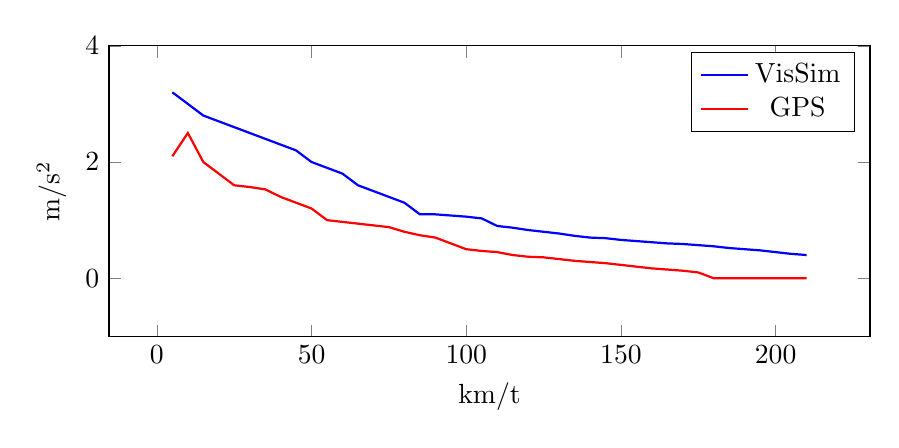
\begin{tikzpicture}
    \begin{axis}
    [
        xlabel=km/t, 
        ylabel=m/s\textsuperscript{2}, 
        ymin=-1, 
        ymax=4,
        width=320,
        height=150
    ]
    \addplot[blue, thick] coordinates 
    {
    	(5, 3.2)
    	(10, 3)
    	(15, 2.8)
	    (20, 2.7)
	    (25, 2.6)
	    (30, 2.5)
	    (35, 2.4)
    	(40, 2.3)
    	(45, 2.2)
    	(50, 2)
    	(55, 1.9)
    	(60, 1.8)
    	(65, 1.6)
	    (70, 1.5)
	    (75, 1.4)
	    (80, 1.3)
	    (85, 1.1)
    	(90, 1.1)
    	(95, 1.08)
    	(100, 1.06)
    	(105, 1.03)
    	(110, 0.9)
    	(115, 0.87)
	    (120, 0.83)
	    (125, 0.8)
	    (130, 0.77)
	    (135, 0.73)
    	(140, 0.7)
    	(145, 0.69)
    	(150, 0.66)
    	(155, 0.64)
    	(160, 0.62)
    	(165, 0.6)
    	(170, 0.59)
	    (175, 0.57)
	    (180, 0.55)
	    (185, 0.52)
	    (190, 0.5)
    	(195, 0.48)
    	(200, 0.45)
    	(205, 0.42)
    	(210, 0.4)
    };
    \addlegendentry{VisSim}
    \addplot[red, thick] coordinates 
    {
    	(5, 2.1)
    	(10, 2.5)
    	(15, 2)
	    (20, 1.8)
	    (25, 1.6)
	    (30, 1.57)
	    (35, 1.53)
    	(40, 1.4)
    	(45, 1.3)
    	(50, 1.2)
    	(55, 1)
    	(60, 0.97)
    	(65, 0.94)
	    (70, 0.91)
	    (75, 0.88)
	    (80, 0.8)
	    (85, 0.74)
    	(90, 0.7)
    	(95, 0.6)
    	(100, 0.5)
    	(105, 0.47)
    	(110, 0.45)
    	(115, 0.4)
	    (120, 0.37)
	    (125, 0.36)
	    (130, 0.33)
	    (135, 0.3)
    	(140, 0.28)
    	(145, 0.26)
    	(150, 0.23)
    	(155, 0.2)
    	(160, 0.17)
    	(165, 0.15)
    	(170, 0.13)
	    (175, 0.1)
	    (180, 0)
	    (185, 0)
	    (190, 0)
    	(195, 0)
    	(200, 0)
    	(205, 0)
    	(210, 0)
    };
    \addlegendentry{GPS}
    \end{axis}
\end{tikzpicture}

Samtidig er der undersøgt af Pihlkjær afgangsprojekt Aalborg Universitet - Vej og Trafikteknik om deceleration for bilister er præcise i VisSim, dette er også gjort ved sammenligning af VisSim data, med GPS data. På figur \ref{GrafForDecelerationVisSimGPS} kan man se, at VisSims deceleration er markant højere end GPS dataen, man ser også at VisSim er lineæret udspillet. Det vurderes at dette kan have betydning for udfaldet i simleringen, hvis VisSims data var nær GPS daten, så ville udfaldet blive mere præcist. Man ser også at VisSims data er konstant, dette betyder at programmet ikke varierer decelerationen i forhold til farten. 

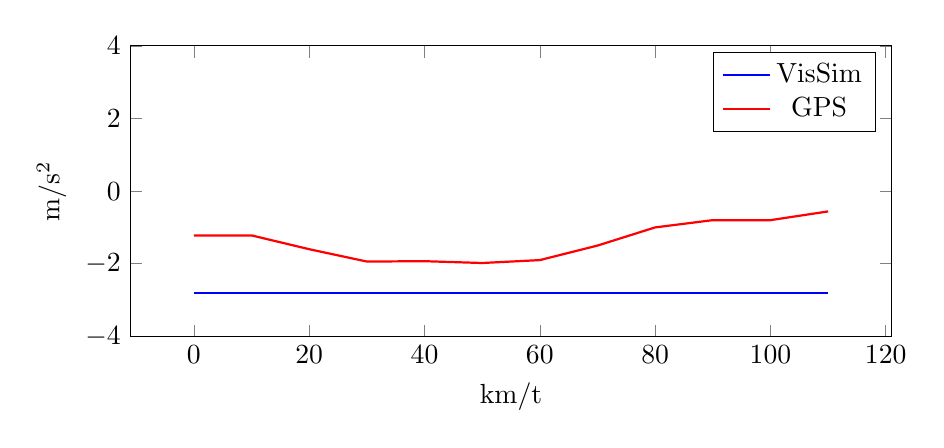
\begin{tikzpicture}
    \begin{axis}
    [
        xlabel=km/t, 
        ylabel=m/s\textsuperscript{2}, 
        ymin=-4, 
        ymax=4,
        width=320,
        height=150
    ]
    \addplot[blue, thick] coordinates 
    {
    	(0, -2.8)
    	(10, -2.8)
	    (20, -2.8)
	    (30, -2.8)
    	(40, -2.8)
    	(50, -2.8)
    	(60, -2.8)
	    (70, -2.8)
	    (80, -2.8)
    	(90, -2.8)
    	(100, -2.8)
    	(110, -2.8)
    };
    \addlegendentry{VisSim}
    \addplot[red, thick] coordinates 
    {
    	(0, -1.22)
    	(10, -1.22)
	    (20, -1.6)
	    (30, -1.94)
    	(40, -1.93)
    	(50, -1.98)
    	(60, -1.9)
	    (70, -1.5)
	    (80, -1)
    	(90, -0.8)
    	(100, -0.8)
    	(110, -0.56)
    };
    \addlegendentry{GPS}
    \end{axis}
\end{tikzpicture}

\subsection{Vudering}
VisSim kan anvendes således, at det kan opstilles til hvilket som helst formål. Dette er en god detalje for VisSim, da brugeren selv kan opstille specifikke scenerier og simuleringer som ikke nødvendigvis er trafik relateret. Dette vurderes til at være godt for vedligeholdelsen, da brugeren selv har muligheden for at opstille scenarier. Dette gør VisSim fremtidssikret, således at udviklerne af VisSim ikke selv skal sørger for vedligeholdelsen.

VisSim er et stort program dette kræver viden omkring anvendelsen af VisSim for at brugeren kan benytte programmet til simulering af trafik. Da VisSim ikke kun er beregnet til trafik simulering, så kræver programmet mange detaljer og viden for brugeren, for at udføre en trafik simulering. Der vurderes at det vil være hjælpsomt for brugeren, hvis brugeren ikke skal anvende tid på at lære et nyt program, men i stedet anvende et program, som kun er egnet specifikt til simulering af trafik. 

Vi har opstillet en tabel over de overvejelser vi har gjort os omkring VisSims fordele og ulemper.

\textbf{ILLEGAL TABLE WAS HERE}

%\begin{table}[]
%\centering
%caption{VisSim Fordele og Ulemper}
%\label{VisSimProsAndCons}
%\begin{tabular}{|1|1|1|1|1|1|}
%		& VisSim Fordele og Ulemper				&								&						   &						    & \\
%Fordele & Kan tilpasses til en givet konteksts	& Brugeren kan programere logik & Vedligeholdes af brugere & Kan give meget præcis data & \\
%Ulemper & Besværligt at sætte sig ind i			& Ikke brugervenligt			&						   &							&
%\end{tabular} 
%\end{table}


